%
% MTransformExamples2.tex
%
% (c) 2019 Prof Dr Andreas Müller, Hochschule Rapperswil
%
\documentclass[tikz,11pt]{standalone}
%
% common.tex
%
% (c) 2020 Prof Dr Andreas Müller, Hochschule Rapperswil
%
\usepackage[T1]{fontenc}
\usepackage[utf8]{inputenc}
\usepackage{amsfonts}
\usepackage{amsmath}
\usepackage{amssymb}
\usepackage{times}
\usepackage{txfonts}
\usepackage{tikz}
\usetikzlibrary{arrows,intersections,math,calc,shapes.geometric,automata}
\usepackage{pgfplots}
\pgfplotsset{compat=1.16}
\usepackage{ifthen}


\begin{document}

\definecolor{blueT}{rgb}{0.6671,0.7594,0.8755}
\definecolor{CadetBlue}{cmyk}{.9,.5,0,.35}
\definecolor{gray}{cmyk}{0,0,0,.5}
\definecolor{orbits}{cmyk}{0,0,0,.7}

\def\s{1.99}
%\def\s{1.79}
%\pgfmathparse{(\s/1.95)*0.32175}
\pgfmathparse{(\s/1.95)*0.32300}
\xdef\pngscale{\pgfmathresult}

\begin{tikzpicture}[>=latex, scale=\s]

\clip (-1.45,-3.55) rectangle (5.05,1.6);

\begin{scope}[]
	\def\s{1.07}
	\def\l{0.9}
	\def\ll{0.9}
	\def\lll{1.1}

	\node(ylm) at (0,0) [scale=\pngscale]{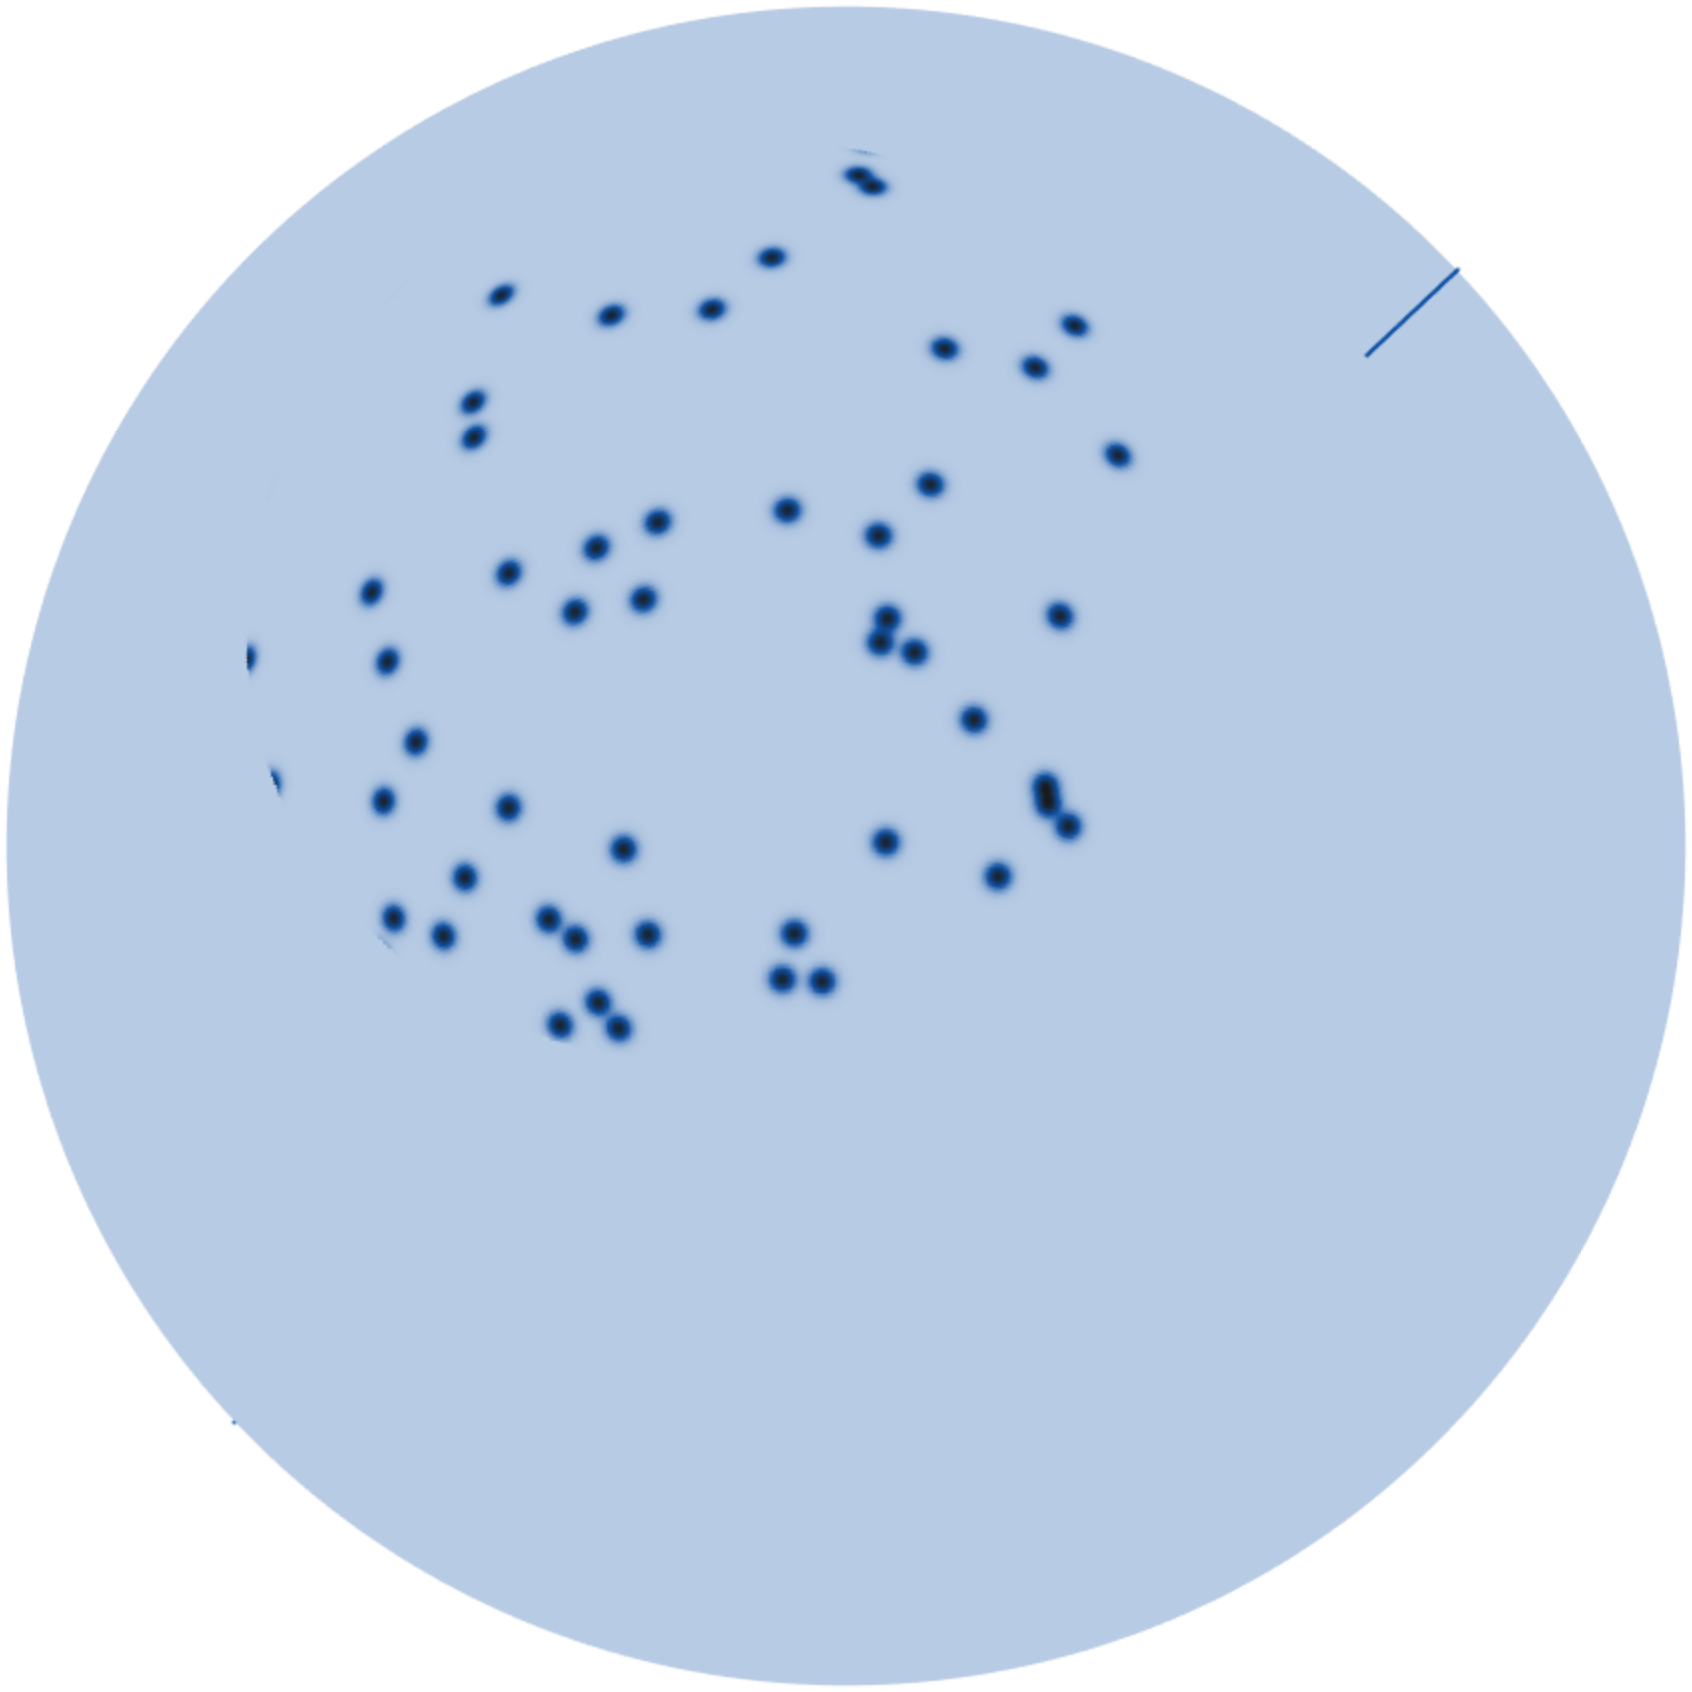
\includegraphics{f.png}};

	\def\r{1.173}
    \draw[black,fill=white,opacity=0,fill opacity=1,ultra thin]({\r*cos(32)},{\r*sin(32)})arc(32:55:\r)--++(0.2,-0.1)--cycle;
    \draw[blueT!85,fill,ultra thin]({\r*cos(32)},{\r*sin(32)})arc(32:55:\r)--++(0,-0.3)--cycle;

	% orbits
	\def\h{0.734}
	\def\ang{180}
	\def\a{0.4}
	\def\b{0.21}
	\draw[orbits,rotate=-46.85,thin] (ylm)++(0,\h) arc(-90:-90+\ang:\a cm and \b cm);
	\draw[orbits,rotate=-46.85,thin] (ylm)++(0,\h) arc(-90:-90-\ang:\a cm and \b cm);
	\def\h{0.373}
	\def\ang{125}
	\def\a{0.7525}
	\def\b{0.4}
	\draw[orbits,rotate=-46.85,thin] (ylm)++(0,\h) arc(-90:-90+\ang:\a cm and \b cm);
	\draw[orbits,rotate=-46.85,thin] (ylm)++(0,\h) arc(-90:-90-\ang:\a cm and \b cm);
	\def\h{-0.03}
	\def\ang{103}
	\def\a{	1.015}
	\def\b{0.54}
	\draw[orbits,rotate=-46.85,thin] (ylm)++(0,\h) arc(-90:-90+\ang:\a cm and \b cm);
	\draw[orbits,rotate=-46.85,thin] (ylm)++(0,\h) arc(-90:-90-\ang:\a cm and \b cm);
	\def\h{-0.429}
	\def\ang{93}
	\def\a{	1.155}
	\def\b{0.6}
	\draw[orbits,rotate=-46.85,thin] (ylm)++(0,\h) arc(-90:-90+\ang:\a cm and \b cm);
	\draw[orbits,rotate=-46.85,thin] (ylm)++(0,\h) arc(-90:-90-\ang:\a cm and \b cm);
	\def\h{-0.776}
	\def\ang{79}
	\def\a{	1.159}
	\def\b{0.61}
	\draw[orbits,rotate=-46.85,thin] (ylm)++(0,\h) arc(-90:-90+\ang:\a cm and \b cm);
	\draw[orbits,rotate=-46.85,thin] (ylm)++(0,\h) arc(-90:-90-\ang:\a cm and \b cm);
	\def\h{-1.03}
	\def\ang{64}
	\def\a{	1.015}
	\def\b{0.53}
	\draw[orbits,rotate=-46.85,thin] (ylm)++(0,\h) arc(-90:-90+\ang:\a cm and \b cm);
	\draw[orbits,rotate=-46.85,thin] (ylm)++(0,\h) arc(-90:-90-\ang:\a cm and \b cm);
	\def\h{-1.16}
	\def\ang{38}
	\def\a{0.76}
	\def\b{0.4}
	\draw[orbits,rotate=-46.85,thin] (ylm)++(0,\h) arc(-90:-90+\ang:\a cm and \b cm);
	\draw[orbits,rotate=-46.85,thin] (ylm)++(0,\h) arc(-90:-90-\ang:\a cm and \b cm);

	% coordinates
	\draw[gray,->, thin](ylm)++({\s*0.86*cos(-26)},{\s*0.86*sin(-26)})--++({\l*0.5*cos(-26)},{\l*0.5*sin(-26)})node[right=-2pt]{$x_2$};
	\draw[gray,->, thin](ylm)++({\s*0.86*cos(-154)},{\s*0.86*sin(-154)})--++({\l*0.5*cos(-154)},{\l*0.5*sin(-154)})node[left=-2pt]{$x_1$};
	\draw[gray,->, thin](ylm)++({\s*0.96*cos(90)},{\s*0.96*sin(90)})--++({\l*0.5*cos(90)},{\l*0.5*sin(90)})node[right=-2pt]{$x_3$};
	\draw[gray,thin](ylm)++({\s*1.096*cos(-90)},{\s*1.096*sin(-90)})--++({\ll*0.22*cos(-90)},{\ll*0.22*sin(-90)});
	\draw[gray,thin](ylm)++({\s*1.096*cos(153.5)},{\s*1.096*sin(153.5)})--++({\ll*0.22*cos(153.5)},{\ll*0.22*sin(153.5)});
	\draw[gray,thin](ylm)++({\s*1.096*cos(26.5)},{\s*1.096*sin(26.5)})--++({\ll*0.22*cos(26.5)},{\ll*0.22*sin(26.5)});

    % axis
    \draw[CadetBlue,very thick](ylm)++({\s*0.934*cos(43.15)},{\s*0.934*sin(43.15)})--++({\lll*0.5*cos(43.15)},{\lll*0.5*sin(43.15)}) node[below right =3pt,xshift = -8pt]{$x$ %fixed point
};
    \draw[CadetBlue,very thick](ylm)++({\s*(-0.934-0.163)*cos(43.15)},{\s*(-0.934-0.163)*sin(43.15)})--++({\lll*(-0.5+0.163)*cos(43.15)},{\lll*(-0.5+0.163)*sin(43.15)});
    \node at (-0.8,1.2) {$f$};

\end{scope}

\begin{scope}[xshift=3.4cm]
	\def\s{1.07}
	\def\l{0.9}
	\def\ll{0.9}
	\def\lll{1.1}

	\node(ylm) at (0,0) [scale=\pngscale]{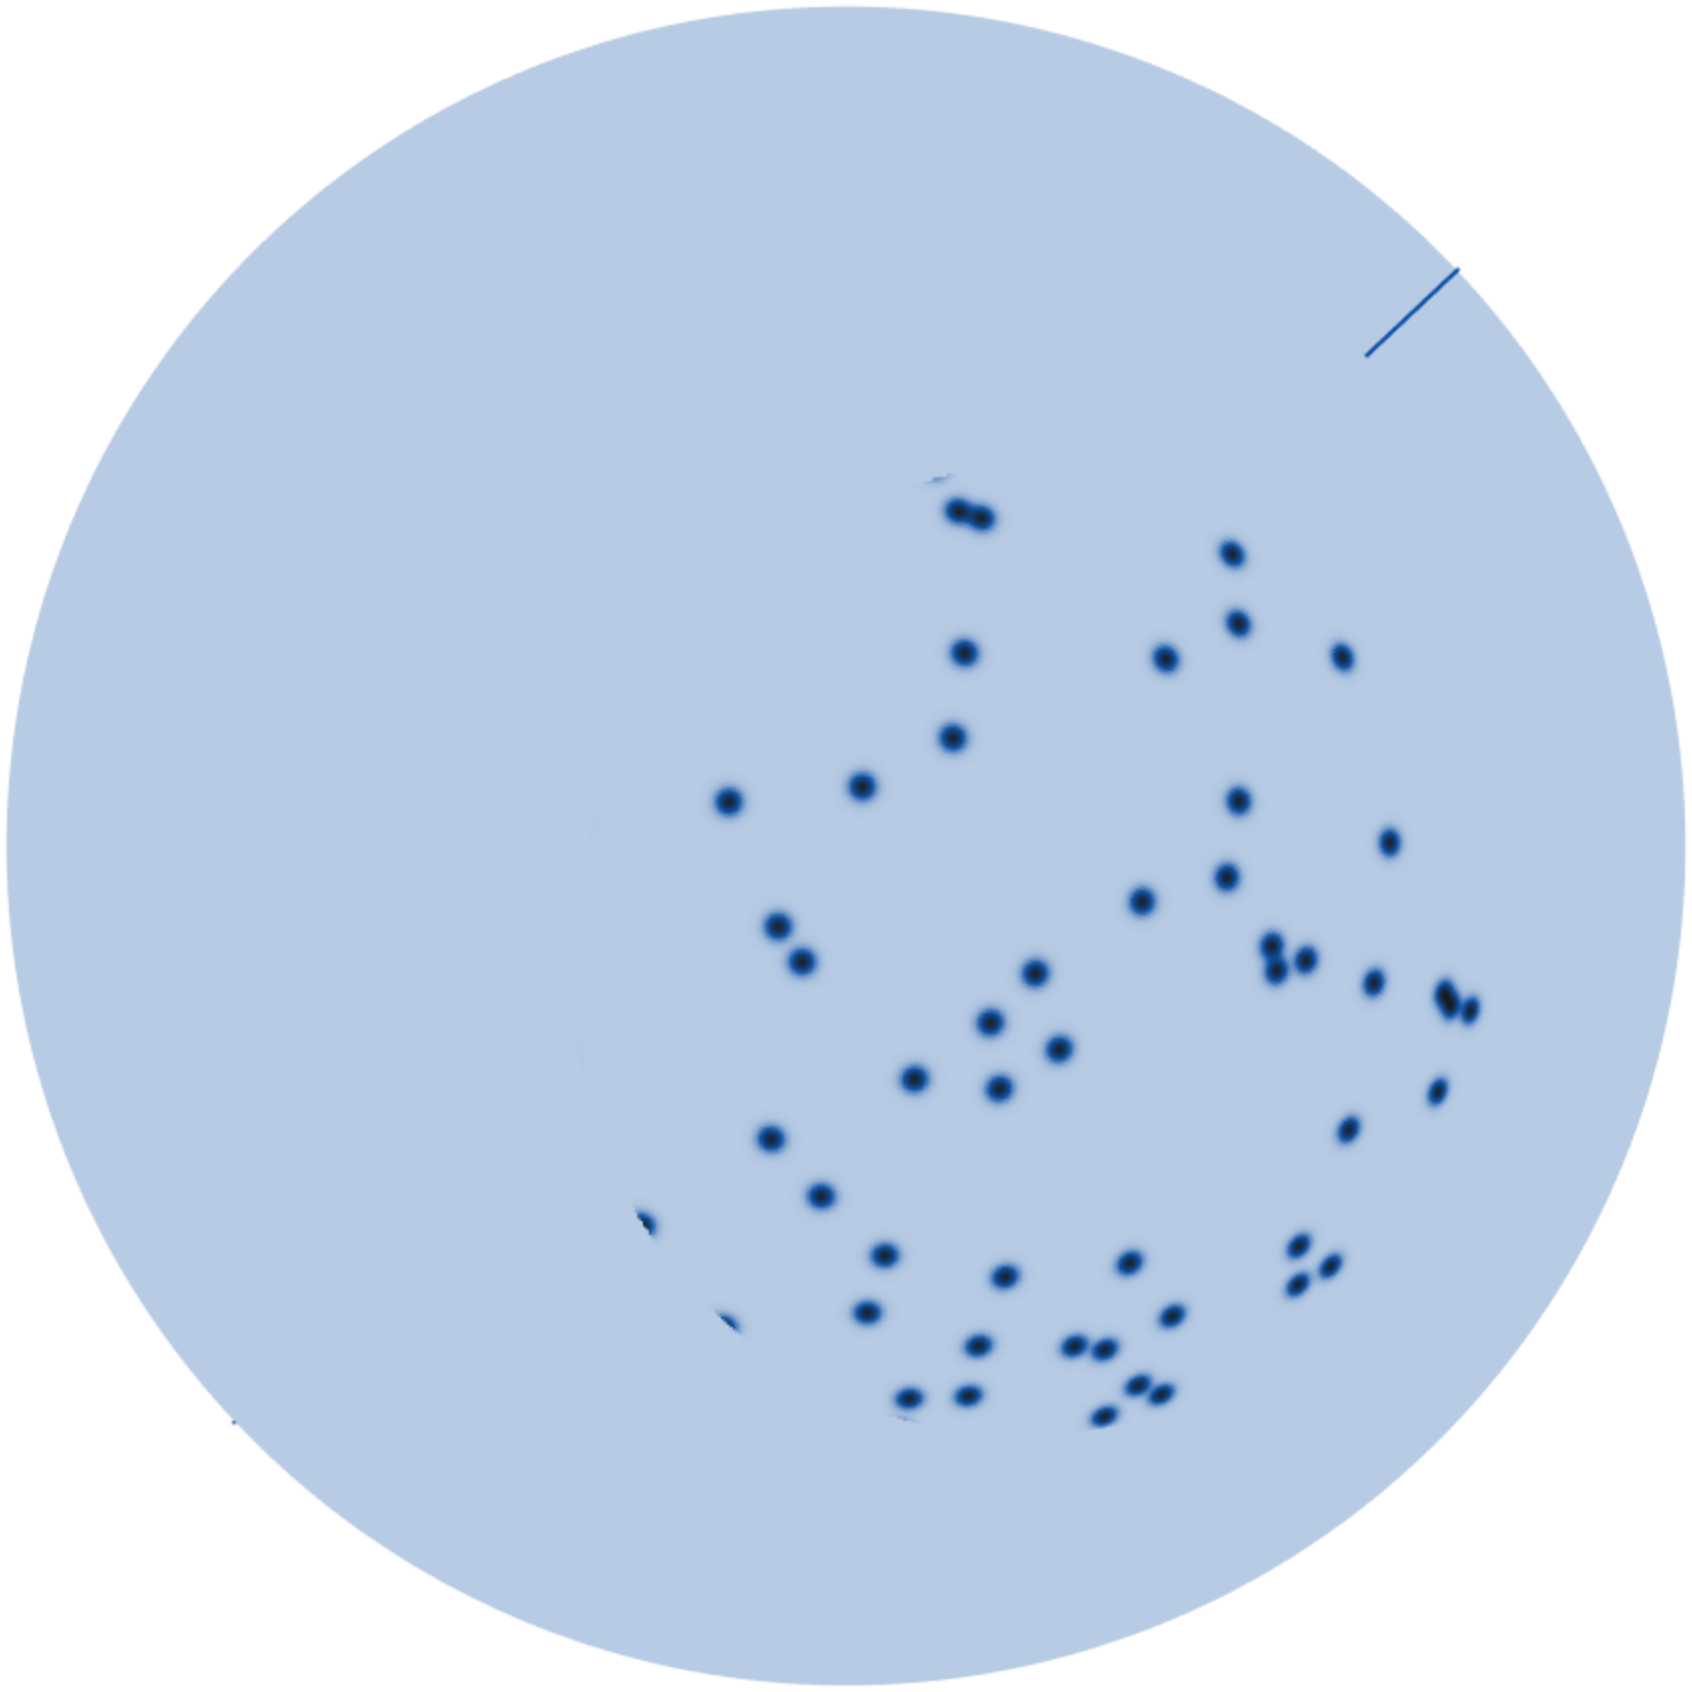
\includegraphics{g.png}};

    \def\r{1.173}
    \draw[black,fill=white,opacity=0,fill opacity=1,ultra thin]({\r*cos(32)},{\r*sin(32)})arc(32:55:\r)--++(0.2,-0.1)--cycle;
    \draw[blueT!85,fill,ultra thin]({\r*cos(32)},{\r*sin(32)})arc(32:55:\r)--++(0,-0.3)--cycle;

	
	% orbits
	\def\h{0.734}
	\def\ang{180}
	\def\a{0.4}
	\def\b{0.21}
	\draw[orbits,rotate=-46.85,thin] (ylm)++(0,\h) arc(-90:-90+\ang:\a cm and \b cm);
	\draw[orbits,rotate=-46.85,thin] (ylm)++(0,\h) arc(-90:-90-\ang:\a cm and \b cm);
	\def\h{0.373}
	\def\ang{125}
	\def\a{0.7525}
	\def\b{0.4}
	\draw[orbits,rotate=-46.85,thin] (ylm)++(0,\h) arc(-90:-90+\ang:\a cm and \b cm);
	\draw[orbits,rotate=-46.85,thin] (ylm)++(0,\h) arc(-90:-90-\ang:\a cm and \b cm);
	\def\h{-0.03}
	\def\ang{103}
	\def\a{	1.015}
	\def\b{0.54}
	\draw[orbits,rotate=-46.85,thin] (ylm)++(0,\h) arc(-90:-90+\ang:\a cm and \b cm);
	\draw[orbits,rotate=-46.85,thin] (ylm)++(0,\h) arc(-90:-90-\ang:\a cm and \b cm);
	\def\h{-0.429}
	\def\ang{93}
	\def\a{	1.155}
	\def\b{0.6}
	\draw[orbits,rotate=-46.85,thin] (ylm)++(0,\h) arc(-90:-90+\ang:\a cm and \b cm);
	\draw[orbits,rotate=-46.85,thin] (ylm)++(0,\h) arc(-90:-90-\ang:\a cm and \b cm);
	\def\h{-0.776}
	\def\ang{79}
	\def\a{	1.159}
	\def\b{0.61}
	\draw[orbits,rotate=-46.85,thin] (ylm)++(0,\h) arc(-90:-90+\ang:\a cm and \b cm);
	\draw[orbits,rotate=-46.85,thin] (ylm)++(0,\h) arc(-90:-90-\ang:\a cm and \b cm);
	\def\h{-1.03}
	\def\ang{64}
	\def\a{	1.015}
	\def\b{0.53}
	\draw[orbits,rotate=-46.85,thin] (ylm)++(0,\h) arc(-90:-90+\ang:\a cm and \b cm);
	\draw[orbits,rotate=-46.85,thin] (ylm)++(0,\h) arc(-90:-90-\ang:\a cm and \b cm);
	\def\h{-1.16}
	\def\ang{38}
	\def\a{0.76}
	\def\b{0.4}
	\draw[orbits,rotate=-46.85,thin] (ylm)++(0,\h) arc(-90:-90+\ang:\a cm and \b cm);
	\draw[orbits,rotate=-46.85,thin] (ylm)++(0,\h) arc(-90:-90-\ang:\a cm and \b cm);

    
	% coordinates
	\draw[gray,->, thin](ylm)++({\s*0.86*cos(-26)},{\s*0.86*sin(-26)})--++({\l*0.5*cos(-26)},{\l*0.5*sin(-26)})node[right=-2pt]{$x_2$};
	\draw[gray,->, thin](ylm)++({\s*0.86*cos(-154)},{\s*0.86*sin(-154)})--++({\l*0.5*cos(-154)},{\l*0.5*sin(-154)})node[left=-2pt]{$x_1$};
	\draw[gray,->, thin](ylm)++({\s*0.96*cos(90)},{\s*0.96*sin(90)})--++({\l*0.5*cos(90)},{\l*0.5*sin(90)})node[right=-2pt]{$x_3$};
	\draw[gray,thin](ylm)++({\s*1.096*cos(-90)},{\s*1.096*sin(-90)})--++({\ll*0.22*cos(-90)},{\ll*0.22*sin(-90)});
	\draw[gray,thin](ylm)++({\s*1.096*cos(153.5)},{\s*1.096*sin(153.5)})--++({\ll*0.22*cos(153.5)},{\ll*0.22*sin(153.5)});
	\draw[gray,thin](ylm)++({\s*1.096*cos(26.5)},{\s*1.096*sin(26.5)})--++({\ll*0.22*cos(26.5)},{\ll*0.22*sin(26.5)});

    % axis
    \draw[CadetBlue,very thick](ylm)++({\s*0.934*cos(43.15)},{\s*0.934*sin(43.15)})--++({\lll*0.5*cos(43.15)},{\lll*0.5*sin(43.15)})node[below=3pt]{$x$};
    \draw[CadetBlue,very thick](ylm)++({\s*(-0.934-0.163)*cos(43.15)},{\s*(-0.934-0.163)*sin(43.15)})--++({\lll*(-0.5+0.163)*cos(43.15)},{\lll*(-0.5+0.163)*sin(43.15)});
    \node at (-0.8,1.2) {$g$};

\end{scope}



\begin{scope}[]



	\begin{scope}[yshift=-3.2cm,scale=1.3]	
%            \node[CadetBlue]at (1.3,0.45){\Huge $ = $};
	
		\draw[->](-1.2,0)--(1.2,0)coordinate[label={$z$}];
		\draw[->](0,0)--(0,1)node[left]{$\mathcal{M}f(x)(z)$};

		\foreach \i in {-1,-0.5,...,1}{
		\draw[very thin](\i,0.05)--(\i,-0.05)node[below]{$\i$};
		}

	\draw[semithick,CadetBlue,rounded corners=0.1pt](-1,0)
	\foreach[count=\i, evaluate=\i as \x using sin(\i-90)] \y in
 {0	,
0	,
0	,
0	,
0	,
0	,
0	,
0	,
0	,
0	,
0	,
0	,
0	,
0	,
0	,
0	,
0	,
0	,
0	,
0	,
0	,
0	,
0	,
0	,
0	,
0	,
0	,
0	,
0	,
0	,
0	,
0	,
0	,
0	,
0	,
0	,
0	,
0	,
0	,
0	,
0	,
0	,
0	,
0	,
0	,
0	,
0	,
0	,
0	,
0	,
0	,
0	,
0	,
0	,
0	,
0	,
0	,
0	,
0	,
0	,
0	,
0	,
0	,
0	,
0	,
0	,
0	,
0	,
0	,
0	,
0	,
0	,
0	,
0	,
0	,
0	,
0	,
0	,
0	,
0	,
0	,
0	,
0	,
0	,
0	,
0	,
0	,
0	,
0	,
0	,
0.0258591382	,
0.2683217815	,
1.7149278105	,
2.8922291327	,
0.7401113611	,
1.8902111985	,
1.8689786438	,
2.7417026276	,
3.4625236733	,
3.0879840213	,
1.6876506471	,
6.5466581302	,
8.8852334367	,
7.5933299575	,
2.6794474444	,
2.298840934	,
0.5104812039	,
2.2988948508	,
1.048684993	,
1.2369546793	,
2.1576978027	,
0.8132701821	,
3.4136412794	,
5.1203954204	,
8.1235036912	,
5.0274102537	,
2.7489621811	,
2.2118500393	,
1.9051151334	,
2.6918690513	,
2.8101661162	,
1.2962050138	,
0.135286236	,
2.8096008798	,
4.4831044568	,
2.7643190225	,
0.9116953617	,
2.3687247148	,
0.9088337591	,
0.0174493319	,
0.0240664437	,
1.7290030736	,
8.0532769306	,
10.4059917321	,
10.8195333782	,
1.5864881544	,
3.7107397241	,
3.1350077808	,
0.1290178597	,
0.0005099225	,
0.0970106727	,
2.1127414758	,
4.5513573402	,
5.3279463776	,
2.4731168795	,
0.1143322266	,
1.3751125047	,
2.0373098322	,
0.1453558868	,
0.0004951307	,
0.0008933205	,
0.2023858682	,
2.2086389929	,
1.2229871227	,
1.61963382	,
2.0700963625	,
2.3864043742	,
1.0530002982	,
0.0233879888	,
2.543966216372E-05	,
1.36713882973544E-09	,
2.9791619896063E-15	,
4.64737583916635E-36	,
0	,
0	,
0	,
0	,
0	,
0	,
0	,
0	,
0	,
0	,
0	,
0	,
0	,
0	,
0	,
0	,
0	,
0}
	{
		--(\x,0.1*\y)
	};


	\end{scope}
	\begin{scope}[xshift=3.4cm,yshift=-3.2cm,scale=1.3]	

		\draw[->](-1.2,0)--(1.2,0)coordinate[label={$z$}];
		\draw[->](0,0)--(0,1)node[left]{$\mathcal{M}g(x)(z)$};

		\foreach \i in {-1,-0.5,...,1}{
		\draw[very thin](\i,0.05)--(\i,-0.05)node[below]{$\i$};
		}

	\draw[semithick,CadetBlue,rounded corners=0.1pt](-1,0)
	\foreach[count=\i, evaluate=\i as \x using sin(\i-90)] \y in
 {0	,
0	,
0	,
0	,
0	,
0	,
0	,
0	,
0	,
0	,
0	,
0	,
0	,
0	,
0	,
0	,
0	,
0	,
0	,
0	,
0	,
0	,
0	,
0	,
0	,
0	,
0	,
0	,
0	,
0	,
0	,
0	,
0	,
0	,
0	,
0	,
0	,
0	,
0	,
0	,
0	,
0	,
0	,
0	,
0	,
0	,
0	,
0	,
0	,
0	,
0	,
0	,
0	,
0	,
0	,
0	,
0	,
0	,
0	,
0	,
0	,
0	,
0	,
0	,
0	,
0	,
0	,
0	,
0	,
0	,
0	,
0	,
0	,
0	,
0	,
0	,
0	,
0	,
0	,
0	,
0	,
0	,
0	,
0	,
0	,
0	,
0	,
0	,
0	,
0	,
0.1199863966	,
0.2666245729	,
1.4984873747	,
2.8945939833	,
0.7418976154	,
1.8889844645	,
1.8610149791	,
2.6536067861	,
3.4582065143	,
3.0822174306	,
1.6765249268	,
6.5584347104	,
8.8831782761	,
7.5997653344	,
2.6890743635	,
2.3028181182	,
0.5126704694	,
2.31594657	,
1.045758258	,
1.2500328933	,
2.1530683039	,
0.802443096	,
3.3969305457	,
5.1193838924	,
8.1141706612	,
5.0537119877	,
2.7677777072	,
2.1982197258	,
1.9093810482	,
2.6772070881	,
2.8081569481	,
1.3001701116	,
0.1406988886	,
2.8251295093	,
4.4889735693	,
2.7544815931	,
0.9242216887	,
2.3748534139	,
0.9036863162	,
0.0173607052	,
0.0253058431	,
1.7389106161	,
8.0516784862	,
10.4336647825	,
10.8135086189	,
1.5932711299	,
3.7085868482	,
3.1454202633	,
0.1317966505	,
0.0005439965	,
0.0998235096	,
2.1090685714	,
4.537736549	,
5.3038285661	,
2.4746027168	,
0.1181221152	,
1.3741911261	,
2.021171145	,
0.1476787143	,
0.000546769	,
0.0009425212	,
0.2042174742	,
2.1941621383	,
1.2323960891	,
1.6228955073	,
2.0665041392	,
2.3874066234	,
1.0535467481	,
0.0237844153	,
0.000026795	,
1.51741147478742E-09	,
3.47658521169568E-15	,
2.63376377512151E-30	,
0	,
0	,
0	,
0	,
0	,
0	,
0	,
0	,
0	,
0	,
0	,
0	,
0	,
0	,
0	,
0	,
0	,
0	}
	{
		--(\x,0.1*\y)
	};


	\end{scope}
\end{scope}

\end{tikzpicture}

\end{document}

